\documentclass[12pt, a4papre]{article}
\usepackage[catalan]{babel}
\usepackage[unicode]{hyperref}
\usepackage{amsmath}
\usepackage{amssymb}
\usepackage{amsthm}
\usepackage{xifthen}
\usepackage{siunitx}
\usepackage{xcolor}
\usepackage{float}
\usepackage{listings}
\usepackage{setspace}
\usepackage{graphicx}
\usepackage{tikz,lipsum,lmodern}
\usepackage[most]{tcolorbox}
\usepackage{circuitikz}
\usepackage{indentfirst}
\usepackage{verbatimbox}
\definecolor{mygreen}{RGB}{28,172,0} % color values Red, Green, Blue
\definecolor{mylilas}{RGB}{170,55,241}
\graphicspath{ {./Fotos/} }

\newcommand{\norm}[1]{\lvert #1 \rvert}

\hypersetup{
    colorlinks = true,
    linkcolor = blue
}

\author{Daniel Vilardell}
\title{Estudi previ practica 5 SSIS}
\date{}

\begin{document}
	\lstset{language=Matlab,%
		frame=single,  
    		%basicstyle=\color{red},
    		breaklines=true,%
    		morekeywords={matlab2tikz},
    		keywordstyle=\color{blue},%
    		morekeywords=[2]{1}, keywordstyle=[2]{\color{black}},
   		 identifierstyle=\color{black},%
    		stringstyle=\color{mylilas},
    		commentstyle=\color{mygreen},%
    		showstringspaces=false,%without this there will be a symbol in the places where there is a space
    		numbers=left,%
    		numberstyle={\tiny \color{black}},% size of the numbers
    		numbersep=9pt, % this defines how far the numbers are from the text
    		emph=[1]{for,end,break},emphstyle=[1]\color{red}, %some words to emphasise
    		%emph=[2]{word1,word2}, emphstyle=[2]{style},    
	}

	\maketitle
	\section{}
	
	\textbf{a)} Sabem que $x[n - n_o] \leftrightarrow X(F)e^{-j2\pi fn_o}$ i ho apliquem per a $n_o= 2$. Tenint en conta que la transformada de una delta $\delta(t - a) \leftrightarrow e^{-j2\pi fa}$ calculem la transformada.
	
	\[
	x[n - 2] \leftrightarrow  \frac{1}{2}e^{j4\pi F} + e^{j2\pi F}  + \frac{3}{2} + e^{-j2\pi F} + \frac{1}{2}e^{-j4\pi F} 
	\]	
	
	I per tant
	\[
	X_d(F) =  (\frac{3}{2} +  cos(4\pi F) + 2cos(2\pi F))e^{-j4\pi F}
	\]
	
	D'aquí podem trobar la seguent taula
	
	\begin{center}
	\begin{tabular}{| c c c c c c c c c |}
	\hline
		F		&0			&1			&-1			&2			&$\frac{1}{2}$		&$-\frac{1}{2}$		&$\frac{1}{3}$		&$\frac{2}{3}$\\ \hline
		$X_d(F)$	&$\frac{9}{2}$	&$\frac{9}{2}$	&$\frac{9}{2}$	&$\frac{9}{2}$	&$\frac{1}{2}$		&$\frac{1}{2}$		&0				&0\\ \hline
	\end{tabular}
	\end{center}
	
	
	\textbf{b)} Si ja que sempre que s'entri una senyal discreta donara lloc a una TF periodica
	
	\section{}
	
	\textbf{a)} Com ja hem vist a la teoria
	\[
	\Pi(\frac{t}{T}) \leftrightarrow Tsinc(Tf)
	\]
	I aplicant la propietat de desplaçament
	\[
	\Pi(\frac{t - \frac{T}{2}}{T}) \leftrightarrow Tsinc(Tf)e^{-j\pi fT}
	\]
	
	\textbf{b)} Aquesta transformada també la hem vist a teoria i sabem que
	\[
	P_L[n] \leftrightarrow \frac{sin(\pi F L)}{sin(\pi F)}e^{-j\pi F(L - 1)}
	\]
	
	\textbf{c)} Les grafiques obtingudes son les següents.
	
	\begin{figure}[H]
		\begin{center}
		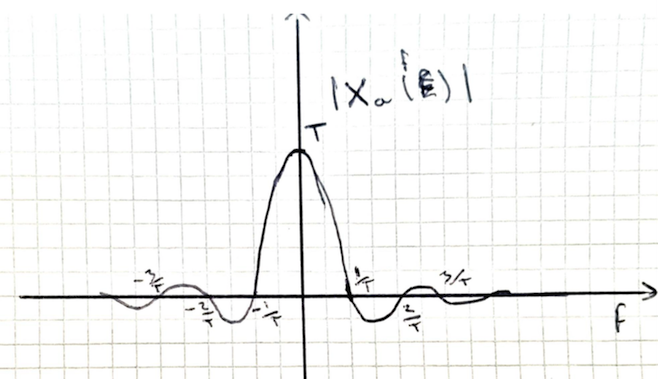
\includegraphics[width=100mm]{SSIS2.png}
		\end{center}
	\end{figure}
	
	\begin{figure}[H]
		\begin{center}
		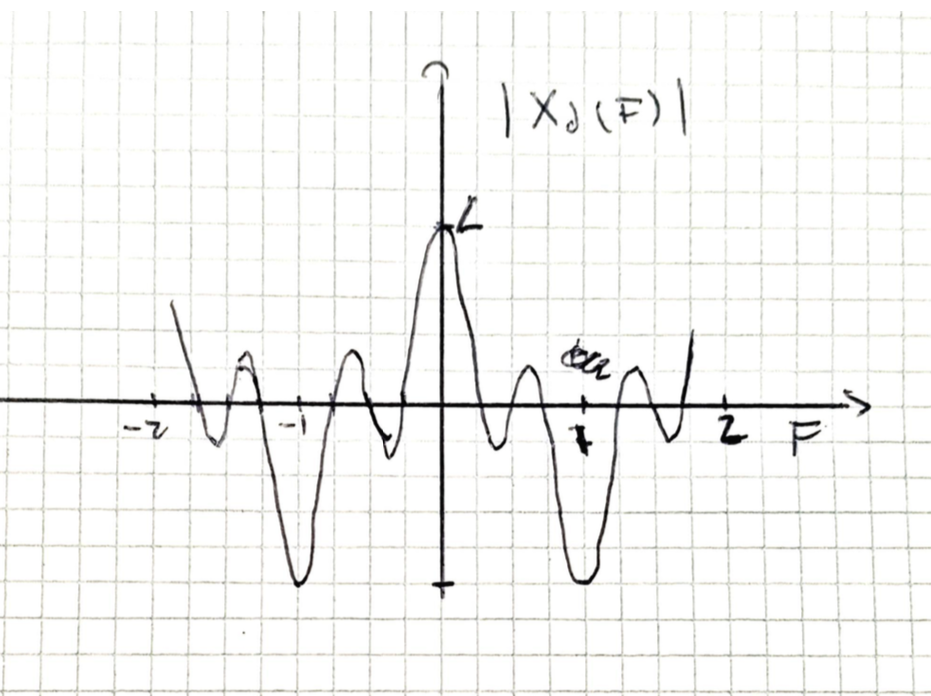
\includegraphics[width=100mm]{SSIS1.png}
		\end{center}
	\end{figure}
	
	\begin{figure}[H]
		\begin{center}
		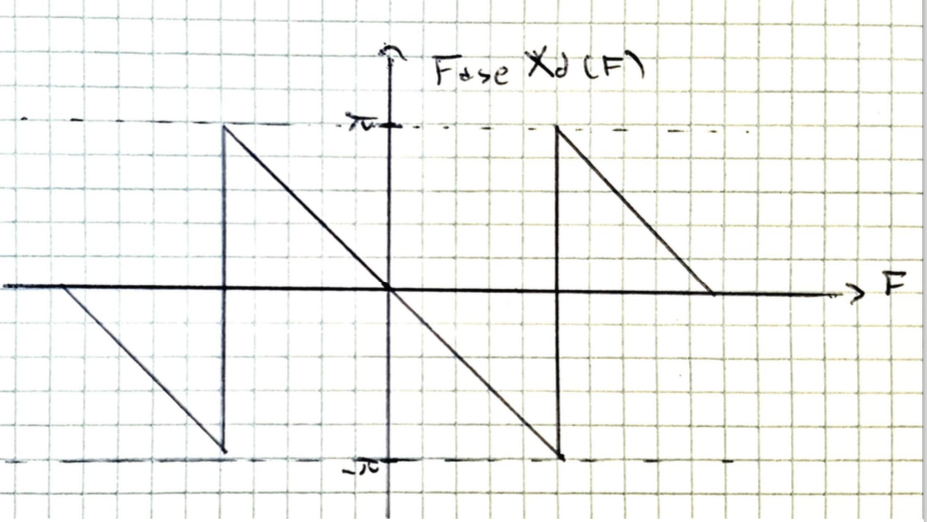
\includegraphics[width=100mm]{SSIS3.png}
		\end{center}
	\end{figure}
	
	\section{}
	
	Per aquesta secció assumirem que l'enunciat era erroni i que la funció $x(t)=e^{-\pi t}u(t)$ i no $x(t)=e^{-\pi}u(t)$ com diu.
	
	\textbf{a)} Sabem per teoria que la transformada de fourier de la exponencial per el pols unitat es
	\[
	x_a(t)=e^{-\pi t}u(t) \leftrightarrow X_a(f) = \frac{1}{\pi+j2\pi f}
	\]
	
	\textbf{b)} Per a calcular aquesta transformada aplicarem la definicio de DFT
	
	\[
	X_d(F) = \sum_{n = -\infty}^{\infty}e^{-\frac{n}{10}}u[n]e^{-j2\pi Fn} = X_d(F) = \sum_{n = 0}^{\infty}e^{n(-\frac{1}{10}-j2\pi F)}
	\]
	\[
	X_d(F) = \frac{1}{1 - e^{-\frac{1}{10}-j2\pi F}}
	\]
	
	\textbf{c)} Si mostregem la senyal $x_a(t)=e^{-\pi t}u(t)$ cada $\frac{1}{10}$ segons obtenim el seguent
	
	\[
	x_a mostrejat[n] = e^{-\pi \frac{n}{10}}u(n) \forall n \in \mathbb{Z} = x_d[n]
	\]
	
	\newpage
	\section{}
	
	\lstinputlisting{DFT.m}
	
\end{document}